\section{The Radon transform method}
\label{sec:Radon}
[TODO: rewrite this paragraph.] The global position angles obtained from the \texttt{kinemetry} method are well defined for coherently rotating stellar or gas velocity fields. In cases where galaxies exhibit radial variation in the velocity fields for example due to warps, where the velocity field in the outer regions is tilted compared with the core, in kinematically decoupled cores (KDCs), in bars or in oval distortions, or in local regions of irregular velocity distribution where the global PA does not provide a clear-cut description of the velocity field, a finer level of detail of the radial variation of the velocity field be accomplished using the Radon transform method. 

The Radon transform (RT) is a mathematical transformation of an image devised to reveal internal properties of an object such as structure. The transform method was originally devised by Johann Radon in 1917 \citep{radon1917determination}. Since then the technique has been applied to many fields, including various branches of astronomy including microwave, radio and x-ray applications. \citet{deans2007radon} describes many of these applications, and also includes an English translation of Radon's original German text. In a more recent treatment  \citet{7910dc8d5b654c90ac4bc94c67d06f01} describes the application of the RT in the field of digital signal processing and presents algorithms for its implementation. For our purposes \cite{2018MNRAS.480.2217S} describe the application of the Radon Transform to galaxy kinematic studies.  

\begin{figure}[h]
    \centering
    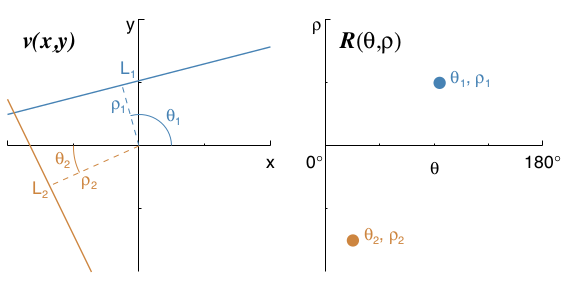
\includegraphics[width=\columnwidth]{images/RadonPlots/Radon-transform-Stark.png}
    \caption{The Radon transform: the figure illustrates the Radon transform and its coordinate system as described in \citet{2018MNRAS.480.2217S}. Line integrals across an image are calculated along all possible lines, parameterised by the coordinates [$\theta$, $\rho$], that cross the 2D function v(x, y). Two examples are shown in the left-hand panel, where the integrals are calculated over the solid lines, L$_1$ and L$_2$, which are perpendicular to the [$\theta, \rho$] vectors and mapped to the points $\theta_1$, $\rho_1$ and $\theta_2$, $\rho_2$ in [$\theta$, $\rho$] parameter space in the right-hand panel. In the Radon transform coordinate system, $\theta$ ranges from 0 to 180 $\deg$ while $\rho$ ranges from $-\infty$ to $\infty$  such that a position below the x-axis corresponds to $\rho < 0$.}
    \label{fig:RadonTransform}
\end{figure}

\citet{2018MNRAS.480.2217S} have applied the Radon transform technique to stellar and gas velocity fields obtained from the MaNGA integral field survey in order to quantify radial variations in the kinematic position angles of galaxies (PA$_k$) using the Radon transform method \citep[see e.g.][]{radon1917determination, 7910dc8d5b654c90ac4bc94c67d06f01}. 
The Radon Transform, $R$, is defined as

\begin{equation}
    \label{eqn:radon}
    R(\rho,\theta)=\int_{L}{v(x,y)\, \diff l},
\end{equation}

where $v(x,y)$ is a 2D velocity field defined in Cartesian coordinates and $\int_{L}$ is the line integral at transform sky-plane polar coordinates ($\rho,\theta$). This transform is illustrated graphically in Fig. \ref{fig:RadonTransform} where lines through an image in 2D velocity space are mapped to a series of points in Radon transform [$\theta,\rho$] space by means of line integrals at various angles about the velocity space axes, and at various distances offset from the velocity space origin. 

\citet{2018MNRAS.480.2217S} apply a modification to the Radon transform, to obtain the \textit{Absolute} Radon Transform, as defined in Eqn. (\ref{eqn:radon}), by taking the integral of the absolute values of the velocity field difference of each point $v(x_i,y_i)$ and the mean of all values along the line segment.

\begin{equation}
    \label{eqn:radon_absolute}
    R_A=\int{| v(x,y) - \langle v(x,y) \rangle | \, \diff l}.
\end{equation}

There is a further variants to the Absolute Radon Transform described by \citet{2018MNRAS.480.2217S} called the \textit{bounded}, or aperture restricted, Radon transform, R\textsubscript{AB}. Briefly, R\textsubscript{AB} involves placing integration limits $(\pm{r_{ap}})$, known as the aperture, on the integral of Equation \ref{eqn:radon_absolute} in order to limit the number of spaxels across a velocity map that will be used in the integration.

These are discussed extensively in their Section XX and illustrated in their Figure 2.


\citet{2018MNRAS.480.2217S} have developed a set of IDL (Interactive Data Language) algorithms to perform the Radon transform on an input array representing a velocity field. The IDL code procedures we use in this work is named \texttt{ds\_radon.pro}.

An example of the graphical output of the Radon transform code \texttt{ds\_radon.pro} as applied to a synthetic velocity field is shown in Fig. \ref{fig:Radon}.

\begin{figure}
    \centering
   	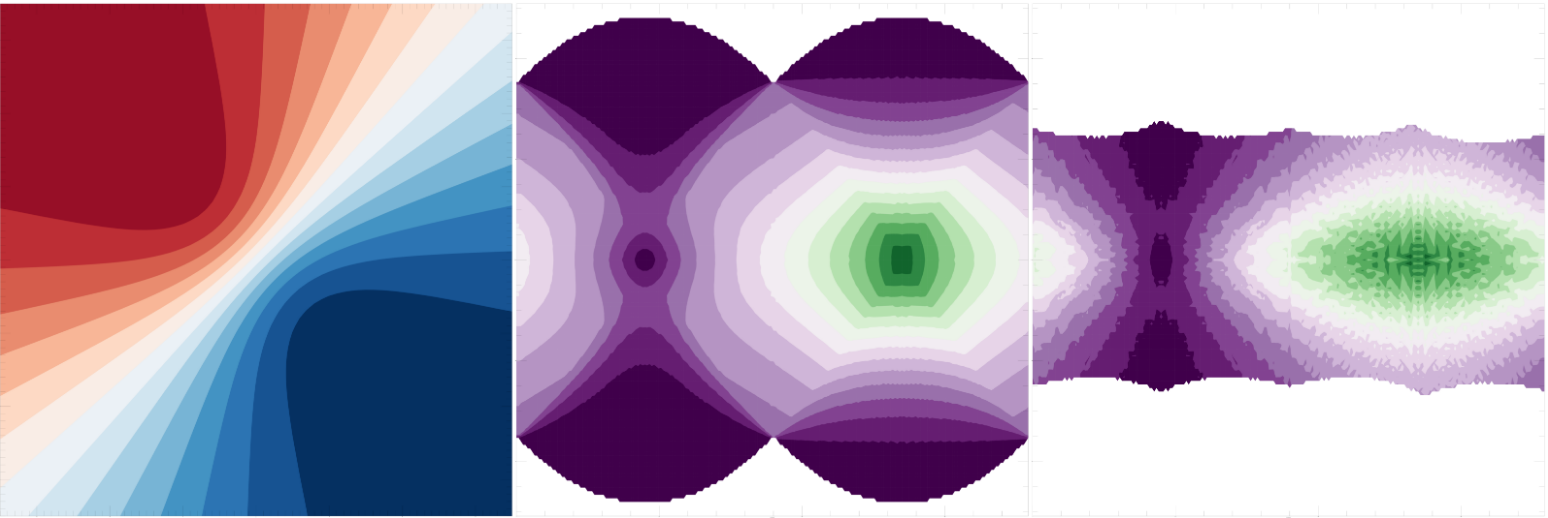
\includegraphics[width=\columnwidth]{images/RadonPlots/example.png}
    \caption{Model Radon transform plots as described in \citet{2018MNRAS.480.2217S}. The left panel shows a synthetic uniform velocity field model, the middle panel shows the the absolute Radon transform of the velocity field and the right panel shows the aperture-restricted absolute transform. We are concerned with the latter, the absolute aperture-restricted  Radon transform of stellar and gas velocity fields in this work.}
    \label{fig:Radon}
\end{figure}

Following \citet{2018MNRAS.480.2217S} we will demonstrate the application of the Radon transform to stellar and gas velocity field data obtained from the SDSS-IV MaNGA integral field survey for a selection of CPSB and RPSB galaxies.  

[This is new method of characterising position angles and how the $\Delta$PA varies within galaxies.]


\begin{figure}
    \centering
   	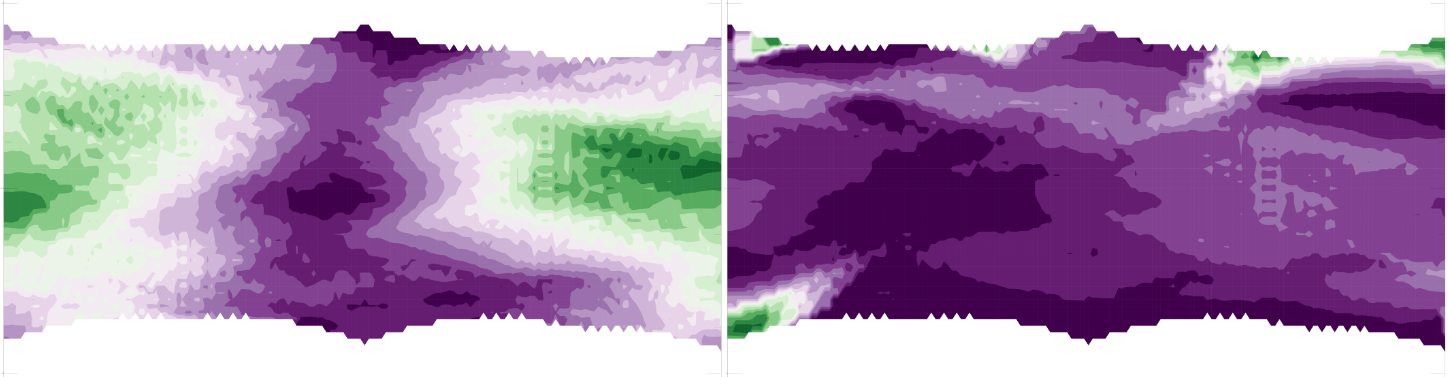
\includegraphics[width=0.8\columnwidth]{images/RadonPlots/RT-snips/CPSB-8313-6101-RT-snip.png}
    \caption{Radon transform plots of the stellar velocity (left panel) and gas velocity (right) fields of CPSB of MaNGA PLATEIFU 8131-6101.}
    \label{fig:RT_8131-6101}
\end{figure}



\begin{figure}
    \centering
    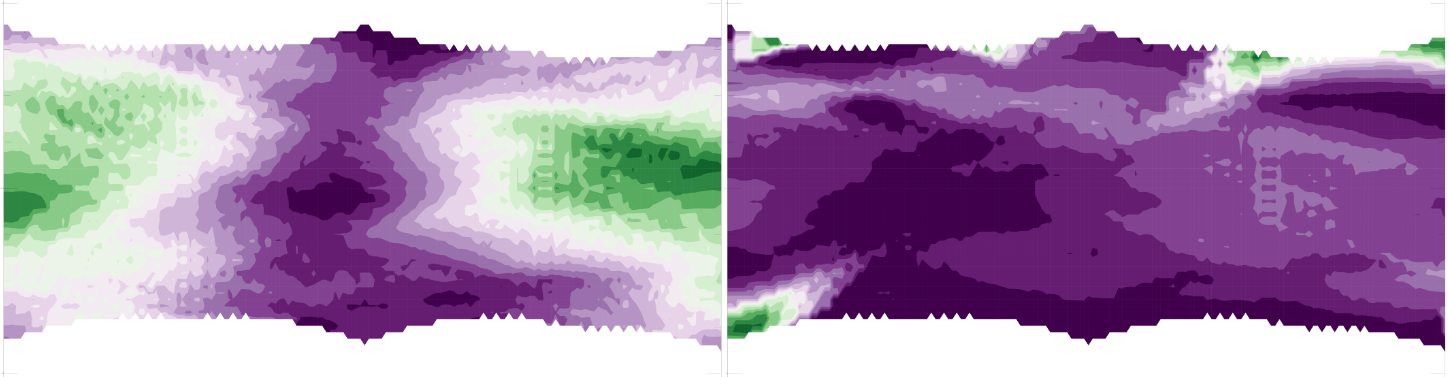
\includegraphics[width=\columnwidth]{images/RadonPlots/RT-snips/CPSB-8313-6101-RT-snip.png}
    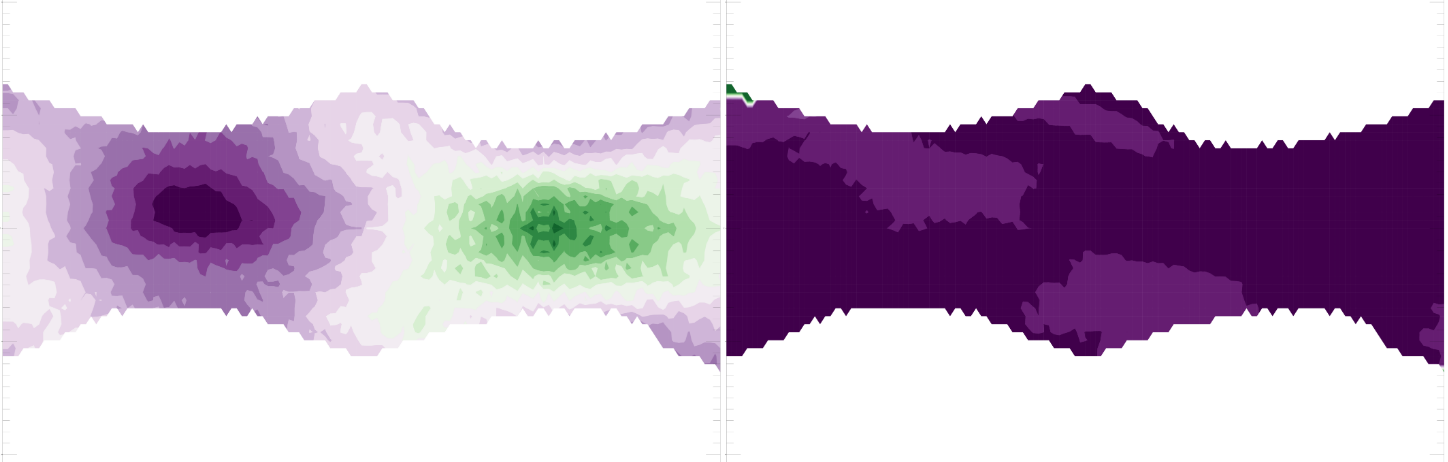
\includegraphics[width=\columnwidth]{images/RadonPlots/RT-snips/CPSB-9494-3701-RT-snip.png}
    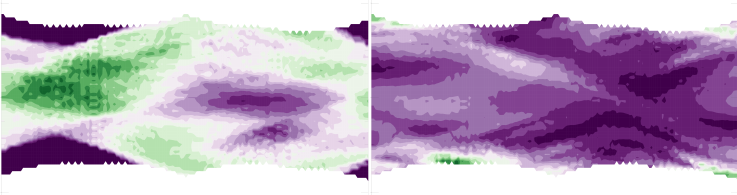
\includegraphics[width=\columnwidth]{images/RadonPlots/RT-snips/CPSB-8398-6102-RT-snip.png}
    \caption{CPSBs: Radon transforms of stellar velocity and gas velocity maps. From the top CPSB-8313-6101, CPSB-9404-3710 and CPSB -8398-6103}
    \label{fig:CPSB-RTs}
\end{figure}

\begin{figure}
    \centering
    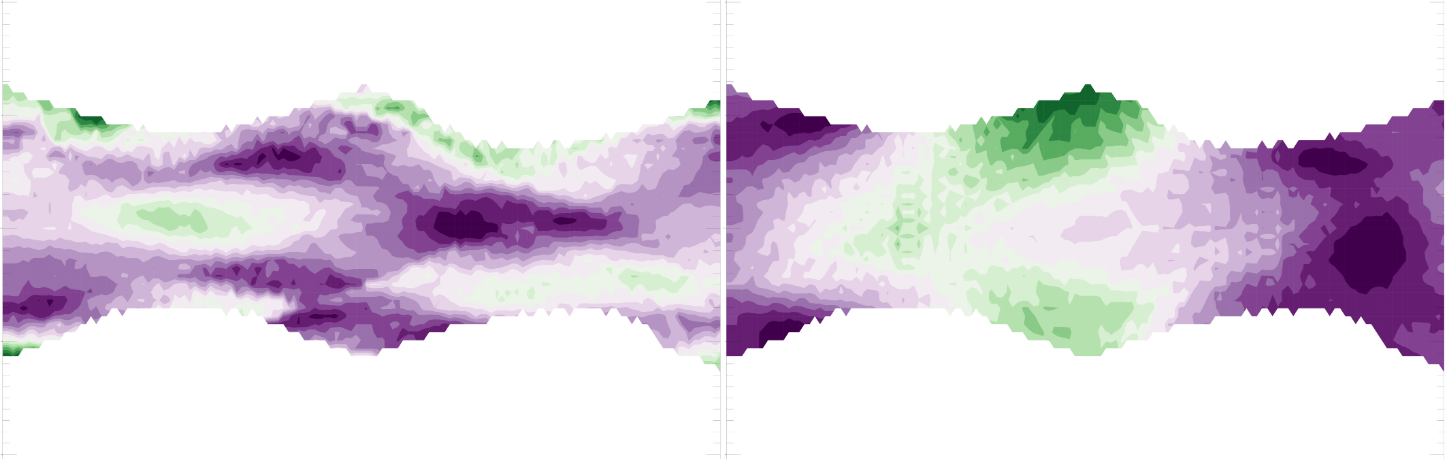
\includegraphics[width=\columnwidth]{images/RadonPlots/RT-snips/RPSB-9872-3701-RT-snip.png}
    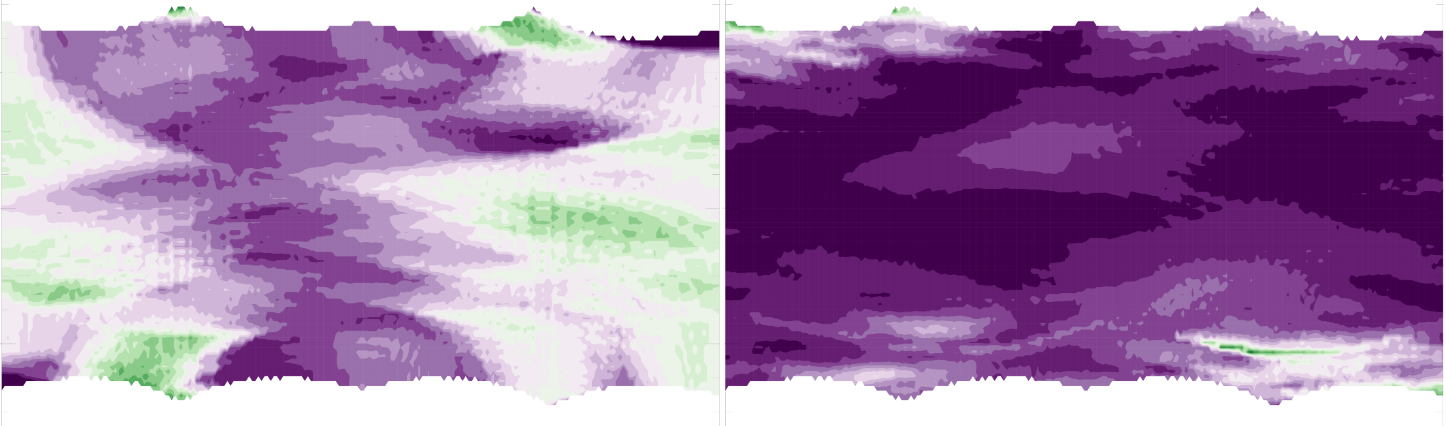
\includegraphics[width=\columnwidth]{images/RadonPlots/RT-snips/RPSB-8932-12704-RT-snip.png}
    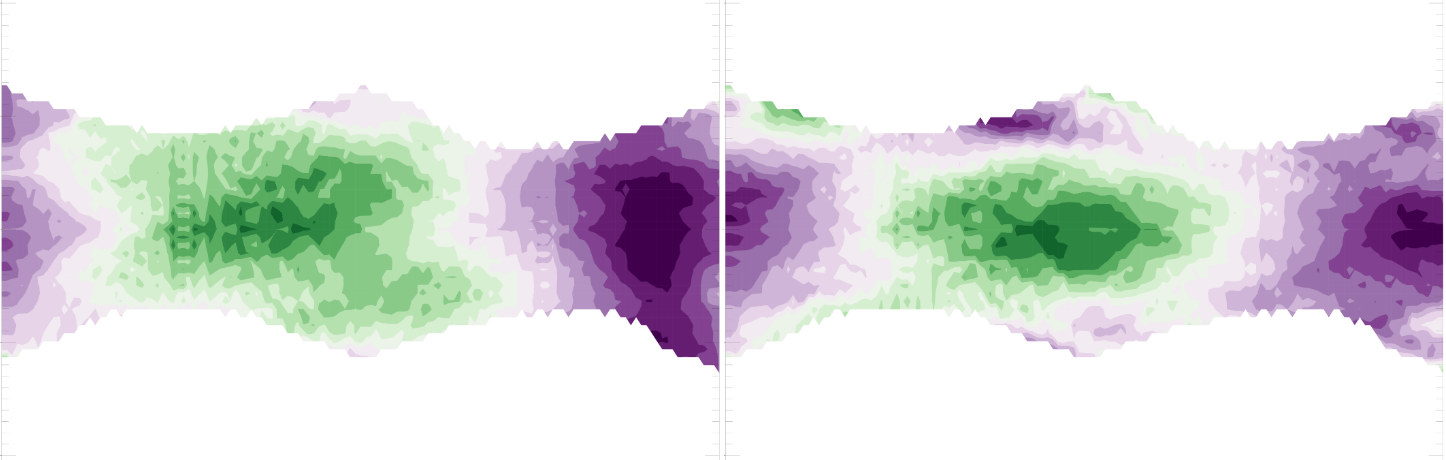
\includegraphics[width=\columnwidth]{images/RadonPlots/RT-snips/RPSB-8554-3701-RT-snip.png}
    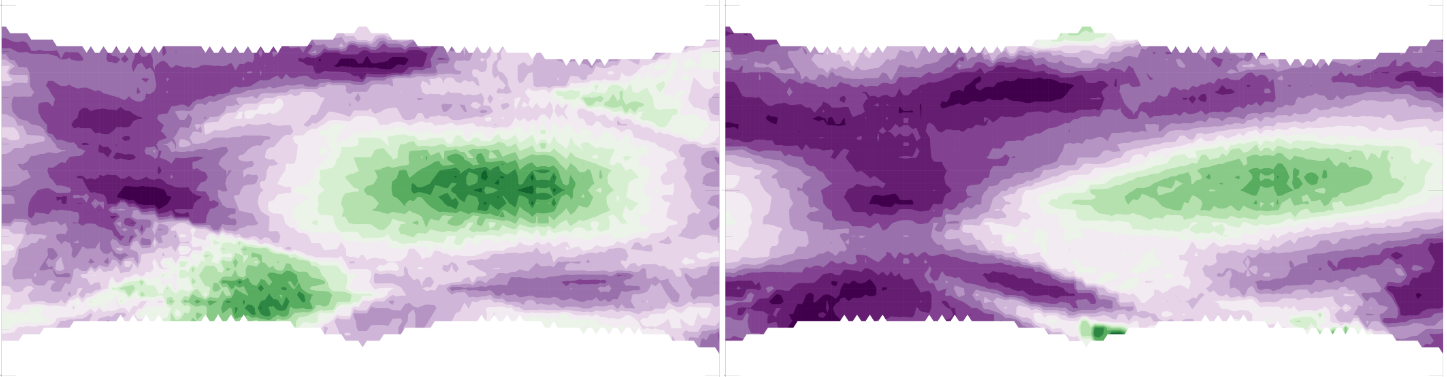
\includegraphics[width=\columnwidth]{images/RadonPlots/RT-snips/RPSB-8323-6103-RT-snip.png}
    \caption{Caption}
    \label{fig:RPSB-RTs}
\end{figure}

\subsection{Radon profile classification procedure}
\label{sec:Radon-classification}

\cite{2018MNRAS.480.2217S} identified 5 commonly recurring patterns in the stellar and gas velocity field Radon transform profiles of their MaNGA galaxy sample. These patterns were used to classify the computed Radon trace profiles. In this project work we adopt the same classification approach for the Radon profiles of our PSB galaxies and their control samples. Simplified models of 4 of the trace profile classes are shown in Figure \ref{fig:class-models}. In addition an asymmetric profile class was identified. Detailed examples of the trace profile class types are presented in Figure 7 of \cite{2018MNRAS.480.2217S}. The salient features of these 5 Radon profile classes are listed below:

\begin{itemize}
    \item Constant, \textbf{Type-C} : Radon profile with relatively constant trace minimum angle $\hat{\theta}$ at all radii $\rho$.
    \item Inner Bend, \textbf{Type-IB} : Galaxies whose Radon profiles exhibit symmetrical variations of $\hat{\theta}$ beginning at $|\rho|=0$, then transitioning to a constant value. 
    \item Outer Bend, \textbf{Type-OB} : Galaxies with constant Radon trace angle $\hat{\theta}$  at small $|\rho|$ which transition to a different value at a greater radius. 
    \item Inner Bend + Outer Bend, \textbf{Type-IB+OB} : Galaxies with Radon profiles showing a combination of the features of Type-IB and Type OB profiles.
    \item Asymmetric, \textbf{Type-A} : The value of the $\hat{\theta}$ varies significantly with $\rho$ across opposite sides of the transform R\textsubscript{AB}. 
 \end{itemize}

\begin{figure}
    \centering
    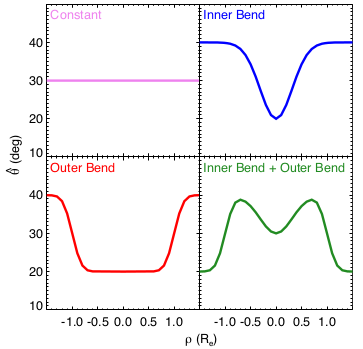
\includegraphics[width=0.8\columnwidth]{images/RadonPlots/Radon-class-models.png}
    \caption[Radon profile class feature identification: toy models]{Toy models of the Radon profile (trace angle minimum $\hat\theta$ versus radius $\rho$). The sub-plots display examples of 4 of the Radon profile classes used for classification of the RT trace plots. Upper left: Constant, Type-C; upper right: Inner Bend, Type-IB; lower left: Outer Bend, Type-OB; and lower right: Inner Bend + Outer Bend, Type-IB+OB. Source: Stark et al. (2018) figure 8.}
    \label{fig:class-models}
\end{figure}

Mathematical functions describing these Radon profile classifications have been identified by \citet[][section 3.6]{2018MNRAS.480.2217S}. This has enabled code routines to be developed which can provide automatic classification of the Radon trace profiles. Results of the automatic classification routines were made available quite late on during the progress of the project work, and therefore were not used extensively in this analysis. Instead, we have adopted a simple visual classification method to categorise each of our sample galaxy into one of the 5 Radon profile trace types listed above. Visual classifications were determined by following a 3-step process:

\begin{enumerate}
    \item Firstly we obtain the MAPS data cube FITS files for the selected PSB galaxies listed in Tables \ref{tab:my-CPSBs} and \ref{tab:my-RPSBs}, and a similar number of 'normal' galaxies drawn from their respective control samples, as described in Section \ref{sec:controls}, downloaded from the MaNGA website.
    \item Next, we process each of data cubes through the Radon transform wrapper code to obtain graphical output files showing the galaxy SDSS $gri$ image cutout, the MaNGA stellar velocity map, the absolute bounded Radon transform R\textsubscript{AB} plot and the Radon profile plot of $\hat{\theta}$ versus $\rho$. An example of this output for the CPSB galaxy 8979-1902 is shown in Figure \ref{fig:CPSB-8979-1902-SNIP}. 
    \item  We then examine the output plot for each galaxy to  visually assess the relative qualitative strength of each of the 5 classification features by assigning a numeric weighting as given in Table \ref{tab:features}. This method adds a semi-quantitative approach to the visual assessment process.
\end{enumerate}

\begin{figure*}
    \centering
    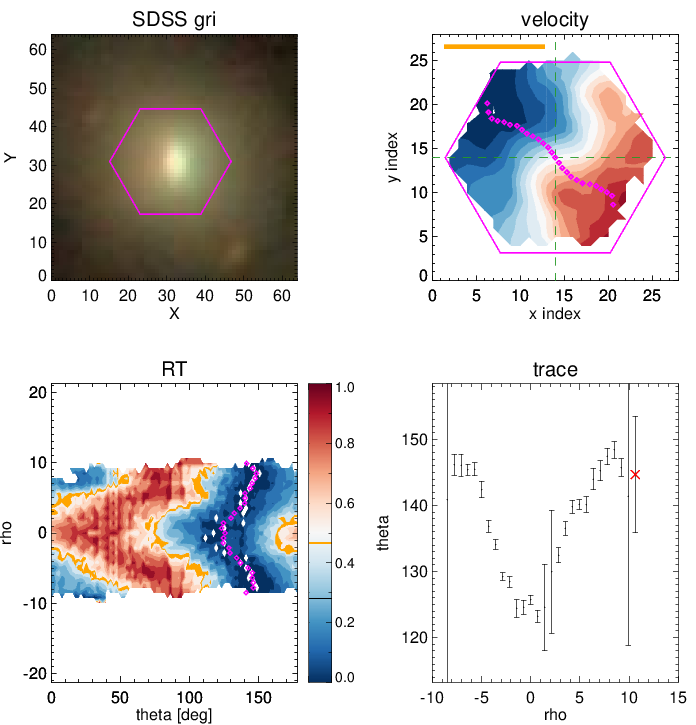
\includegraphics[width=0.8\textwidth]{images/RadonPlots/RT-SNIPS-NEW/CPSB-8979-1902-SNIP.png}
    \caption[Radon transform code output graphics for the CPSB 8979-1902]{Radon transform code output graphics for the CPSB 8979-1902. Top left: SDSS gri image cutout, Top right: stellar velocity map with kinematic position angle (PA$_{k}$) shown as the magenta line, lower left: Radon transform (RT) of the stellar velocity field with the transform minimum angle $\hat\theta$ plotted across radius $\rho$ in magenta, lower right: the Radon profile trace of the RT minimum.}
    \label{fig:CPSB-8979-1902-SNIP}
\end{figure*}

\begin{table}
    \caption[Relative weighting of Radon profile feature strengths used in visual classification]{Relative weighting of Radon profile feature strengths used for the visual classification of Radon profile feature types: Constant, Inner Bend, Outer Bend, Inner Bend + Outer Bend or Asymmetric. The weighting is assigned to help quantify the visual appearance of the trace profile plots.}
    \label{tab:features}
    \centering
    \begin{tabular}{cl}
    \hline
    Value & Visual appearance \\
    \hline
    2 & The feature is visually predominant \\
    1 & Some evidence of the feature is apparent \\
    0 & The feature is absent \\
    \hline
    \end{tabular}
\end{table}

The Radon output graphic plots for 127 galaxies (PSBs and some of control sets) were visually assessed in alphanumerical order of their PLATEIFU file name tag, which effectively creates a random sequence across the groups. Classifying the galaxies in each group sequentially may have led to preferential identification of similar features in that group, thereby introducing a classification bias.

The Radon transform output plots for each galaxy were inspected to make an assessment of the visual strength of each of the Radon profile type features evident. A numerical value 0, 1 or 2, representing the visual strength of apparent features from Table \ref{tab:features}, was assigned to each of the 5 predefined Type classes for the galaxy. Based on the relative strength values allocated, a predominant feature Type (C, IB, OB, IB+OB or A) was assigned to that particular galaxy. To determine the relative predominance of Type-IB+OB features we simply summed the strength values assigned to Types IB and OB together. 
In many cases there was ambiguity in the absolute Type assessment, where we had difficulty to select only one of the 5 predefined classes. In these cases a secondary assessment was made, generally this was the most prevalent Type plus a sub-dominant feature. The secondary assessment was intended to be used later to refine the analysis process. 

As a demonstration of the Radon profile visual classification method we select the example of the spiral galaxy 8979-12701. The Radon transform and Radon profile trace for this galaxy are shown in Figure \ref{fig:OB+IB}. Comparing the Radon trace profile with the model traces in Figure \ref{fig:class-models} and the examples given in  Figure 7 of \cite{2018MNRAS.480.2217S}, the visual classification process identified the strength of the features as: C = 1, IB = 2, OB = 2, IB+OB = 2+2 = 4, and A=0. This trace profile is comparable to the Type-OB+IB model and consequently the Radon profile of this galaxy is categorised as Type-OB+IB.

The classification process outlined above was carried out independently by 2 persons in an endeavour to provide some means of eliminating personal subjectivity. The intent is similar  to that adopted by the Galaxy Zoo project which used large-scale public collaboration to classify galaxy morphology \citep{2017MNRAS.464.4176W}. The galaxy-by-galaxy Radon profile Type classifications determined by the two assessors are listed in Tables \ref{tab:full-visual-classification} and \ref{tab:visual-classification-B} in Appendix \ref{sec:visual-classification-tables}.

\begin{figure}
    \centering
    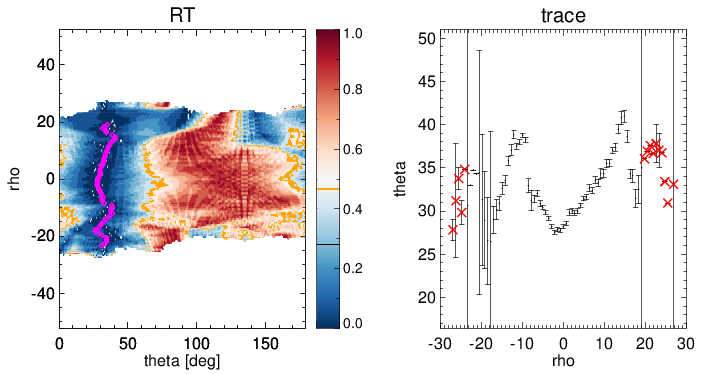
\includegraphics[width=\columnwidth]{images/RadonPlots/RT-SNIPS-NEW/8979-12701-VA-OB+IB.png}
    \caption[Example of the Radon profile visual classification of galaxy 8979-12701]{Example of the Radon profile visual classification method for galaxy 8979-12701. The Radon transform (RT) plot is shown in the left panel and the Radon profile trace on the right. The RT plot minimum (magenta line) shows an indication of a wide outer bend (OB) feature. The trace plot also shows a narrower inner bend (IB) feature centred at radius $\rho=0$. We therefore classify the Radon profile of this galaxy as Type-OB+IB.}
    \label{fig:OB+IB}
\end{figure}

During the classification assignment exercise  some difficulties were encountered mainly with Radon trace profiles that did not fit easily into on of the 5 classification Types. An example of this is seen in the case of 8555-3701 where a clearly defined Inner Bend appears superimposed on an asymmetric trace as shown in Figure \ref{fig:8555-3701-A+IB}. The form of this trace does not fall readily into either of the Type-A or Type-IB categories, however faced with a choice of Types, and a requirement to select only one of the 5 categories, the natural choice was to opt for the predominant feature, in this case Type-A, asymmetric. The reader may disagree and opt for Type-IB, or even Type-OB+IB. This demonstrates the challenges encountered in the visual classification of Radon profiles.

\begin{figure}
    \centering
    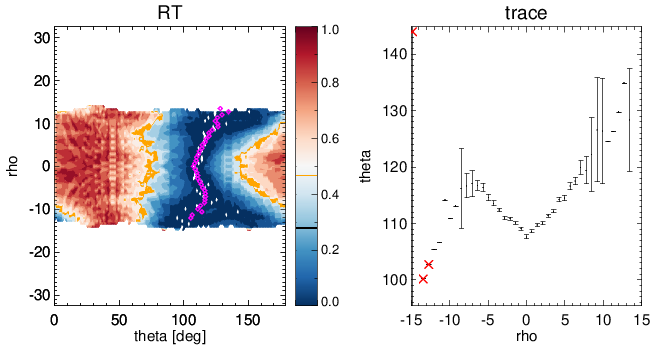
\includegraphics[width=\columnwidth]{images/RadonPlots/RT-SNIPS-NEW/8555-3701-A+IB.png}
    \caption[Radon transform and profile trace plots for the galaxy 8555-3701]{Radon transform and profile trace plots for the galaxy 8555-3701. An inner bend appears superimposed on a generally asymmetric trace.}
    \label{fig:8555-3701-A+IB}
\end{figure}

In many other cases bends, or detectable velocity field disturbances, are evident as notches at well off-centre radii on otherwise constant or largely asymmetric traces. To obtain a comprehensive census at this level of detail these sub-dominant and off-centre features should be taken into account in a secondary analysis as mentioned above. Other than presenting a listing of the mixed secondary classifications obtained by classifier A in Table \ref{tab:full-visual-classification}, we did not pursue a more detailed secondary analysis in this present work.






%% RT-plots-new.tex
%% Images from the new Radon output 

\begin{figure*}
    \centering
    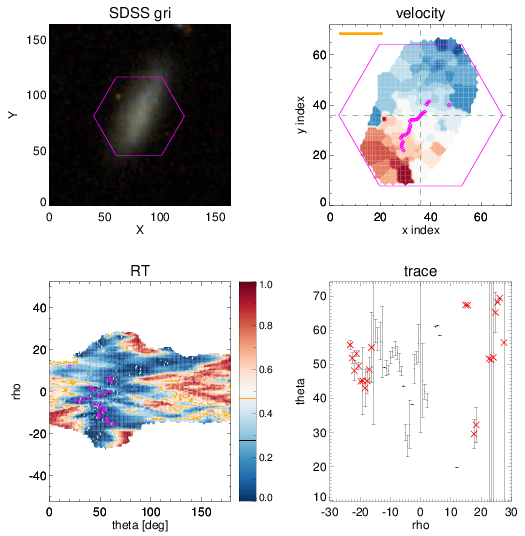
\includegraphics[width=12cm]{images/RadonPlots/RT-SNIPS-NEW/RT-CPSB-9493-12705-SNIP.png}
    \caption{Absolute Radon transform plots of the stellar velocity field of the CPSB MaNGA PLATEIFU 9493-12705. The panels show: top left - the SDSS gri image cutout; top right - the stellar velocity field. The orange coloured  bar in the upper left indicates the Radon aperture size in spaxels; bottom left - the re-scaled Radon transform. The locus of the minimum of the transform is plotted in magenta; and bottom right: the Radon trace plot. The technical details of the RT and Trace plots are described in the text.}
    \label{fig:RT-CPSB-9493-12705-SNIP}
\end{figure*}



